%!TEX root = ../research_overview.tex

\section{Compute within Data Movement}

\subsection{Unified Interface}

\begin{frame}{Photonics-Enabled Data Processing}

    \only<1-1|handout:0>{\centering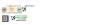
\includegraphics[width=\textwidth]{fig/pho-comp-1.pdf}}%
    \only<2-2>{\centering\includegraphics[width=\textwidth]{fig/pho-comp-2.pdf}}%
    \note<1-1>[item]{I extended this integrated photonics platform beyond classical data communications into the realm of computing accelerators.}
    \note<2-2>[item]{The goal here is to perform some data processing operations right at where the data resides.}
    \note<2-2>[item]{And, by having this unified photonic chiplet that can perform both data movement and data processing, we can reduce the need for shuttling data back and forth between the processor and the memory, but also be able to provide the high bandwidth when it is really needed.}


\end{frame}

\subsection{Photonic MAC}

\begin{frame}{Photonic Multiply-Accumulate (MAC) Accelerators}

    \only<2-2>{\centering\includegraphics[width=0.4\textwidth]{fig/matrix_compressed.pdf}}%
    \note<1-1>[item]{I'll give one example of my research in this direction, which is a photonic multiply-accumulate engine, or photonic MAC.}
    \note<2-2>[item]{Because MAC operations are essential for matrix multiplication, which is widely found in AI/machine learning and digital signal processing applications, it has drawn great attention for making accelerators for these operations, including using integrated photonics.}
    \note<2-2>[item]{And, this work that I'm going to talk about, differs from those existing photonic MAC engines by preserving the full digital precision of the MAC operation. And I'll show you how.}

\end{frame}

\begin{frame}{Existing Solutions Limited in Bit Precision}
    \only<1-1|handout:0>{\centering\includegraphics[width=0.9\textwidth]{fig/mac-limit-1_compressed.pdf}}%
    \only<2-2|handout:0>{\centering\includegraphics[width=0.9\textwidth]{fig/mac-limit-2_compressed.pdf}}%
    \only<3-3>{\centering\includegraphics[width=0.9\textwidth]{fig/mac-limit-3_compressed.pdf}}%
    \vspace{-1em}%
    \begin{center}%
        \fullcite{taitMicroringWeightBanks2016}%
    \end{center}%
    \note<1-1>[item]{Let's first take a look at a typical photonic MAC accelerator today using this architecture called a microring weight bank.}
    \note<2-2>[item]{Suppose we want to do a MAC operation like this. How this traditional architecture works is that, it encodes the multiplicand as an analog light intensity, and encodes the multiplier as an analog voltage applied to the microring, to control how much of a portion of that light can pass through.}
    \note<3-3>[item]{And as you may have noticed, this traditional approach requires converting these digitally stored numbers into the analog domain, and photonic devices aren't  actually good at precisely represent these analog values becaubese they're prone to fabrication and environmental perturbations. This limitation also applies to those architectures using a mesh of Mach-Zehnder interferometers, which encodes the numbers into an analog phase shift. And as a result, these methods are often limited in bit precision that they can achieve.}
\end{frame}

\begin{frame}{Photonic MAC with Full Digital Precision}

    \only<1-1|handout:0>{\centering\includegraphics[width=0.9\textwidth]{fig/dac-1_compressed.pdf}}%
    \only<2-2|handout:0>{\centering\includegraphics[width=0.9\textwidth]{fig/dac-2_compressed.pdf}}%
    \only<3-3|handout:0>{\centering\includegraphics[width=0.9\textwidth]{fig/dac-3_compressed.pdf}}%
    \only<4-4>{\centering\includegraphics[width=0.9\textwidth]{fig/dac-4_compressed.pdf}}%
    \vspace{0.25em}%
    \begin{center}%
        \onslide<1->{\tiny Nauman, N., Robinson, J., \textbf{Wang, Y.} \emph{et al.} in \emph{OFC}, (2025)}%
    \end{center}%
    \note<1-1>[item]{What's unique about our approach is that, we operate the photonic devices in the digital domain.}
    \note<2-2>[item]{And, leveraging our capability of having massive wavelengths channels, we directly look at each bit place of the MAC operation, and assign each digit contributing to this bit place a unique wavelength.}
    \note<3-3>[item]{Now, to get the MAC result of this bit place becomes counting the number of ones on this bus, where a one would let the light pass and a zero would block the light. So, this counting can be performed instantaneously by this analog photodetector at the end of this bus waveguide.}
    \note<3-3>[item]{This is where the acceleration comes from, because, we don't need to rely on using a bunch of adders to do the counting, so basically the larger the operation, the better gain in acceleration we can get.}
    \note<3-3>[item]{And this is why this architecture is uniquely enabled by our Kerr-comb driven DWDM, where we can have a large number of wavelength channels for this bit counting.}
    \note<4-4>[item]{And here I'm showing some experimental results from a bus waveguide with 8 microrings, and we can see that, since we are operating the microrings in a digital fashion, the output from this analog PD is really distinctive for different number of ones that are being counted.}

\end{frame}

\begin{frame}{Photonic ADC for MAC Result}

    \only<1-1|handout:0>{\centering\includegraphics[width=0.9\textwidth]{fig/adc-1_compressed.pdf}}%
    \only<2-2>{\centering\includegraphics[width=0.9\textwidth]{fig/adc-2_compressed.pdf}}
    \vspace{-1em}%
    \begin{center}%
        \onslide<1->{\tiny Nauman, N., Robinson, J., \textbf{Wang, Y.} \emph{et al.} in \emph{OFC}, (2025)}%
    \end{center}%
    \note<1-1>[item]{So the next step is to convert this analog PD output back into digital domain. And the least significant bit of the result will be the MAC output for this bit place, and the more significant bits will be the carry bits to higher bit places. And we can also do this in the optical domain, reusing this DWDM bus architecture.}
    \note<2-2>[item]{So, by biasing each of these microrings incrementally away from their resonance wavelengths, this same voltage applied to them will only flip a subset of the microrings, like shown in this plot, depending on the input voltage level. This is essentially doing a discretization of the input voltage using a cascaded microring bus.}
    \note<2-2>[item]{So this architecture really keeps both the input and output of the MAC operation in the digital domain while delegating the job of keeping the bit precision to leveraging more parallel wavelengths.}

\end{frame}

\subsection{Continued Scaling}

\begin{frame}{AI Scaling while Bending the Energy Curve}
    \only<1-1|handout:0>{\centering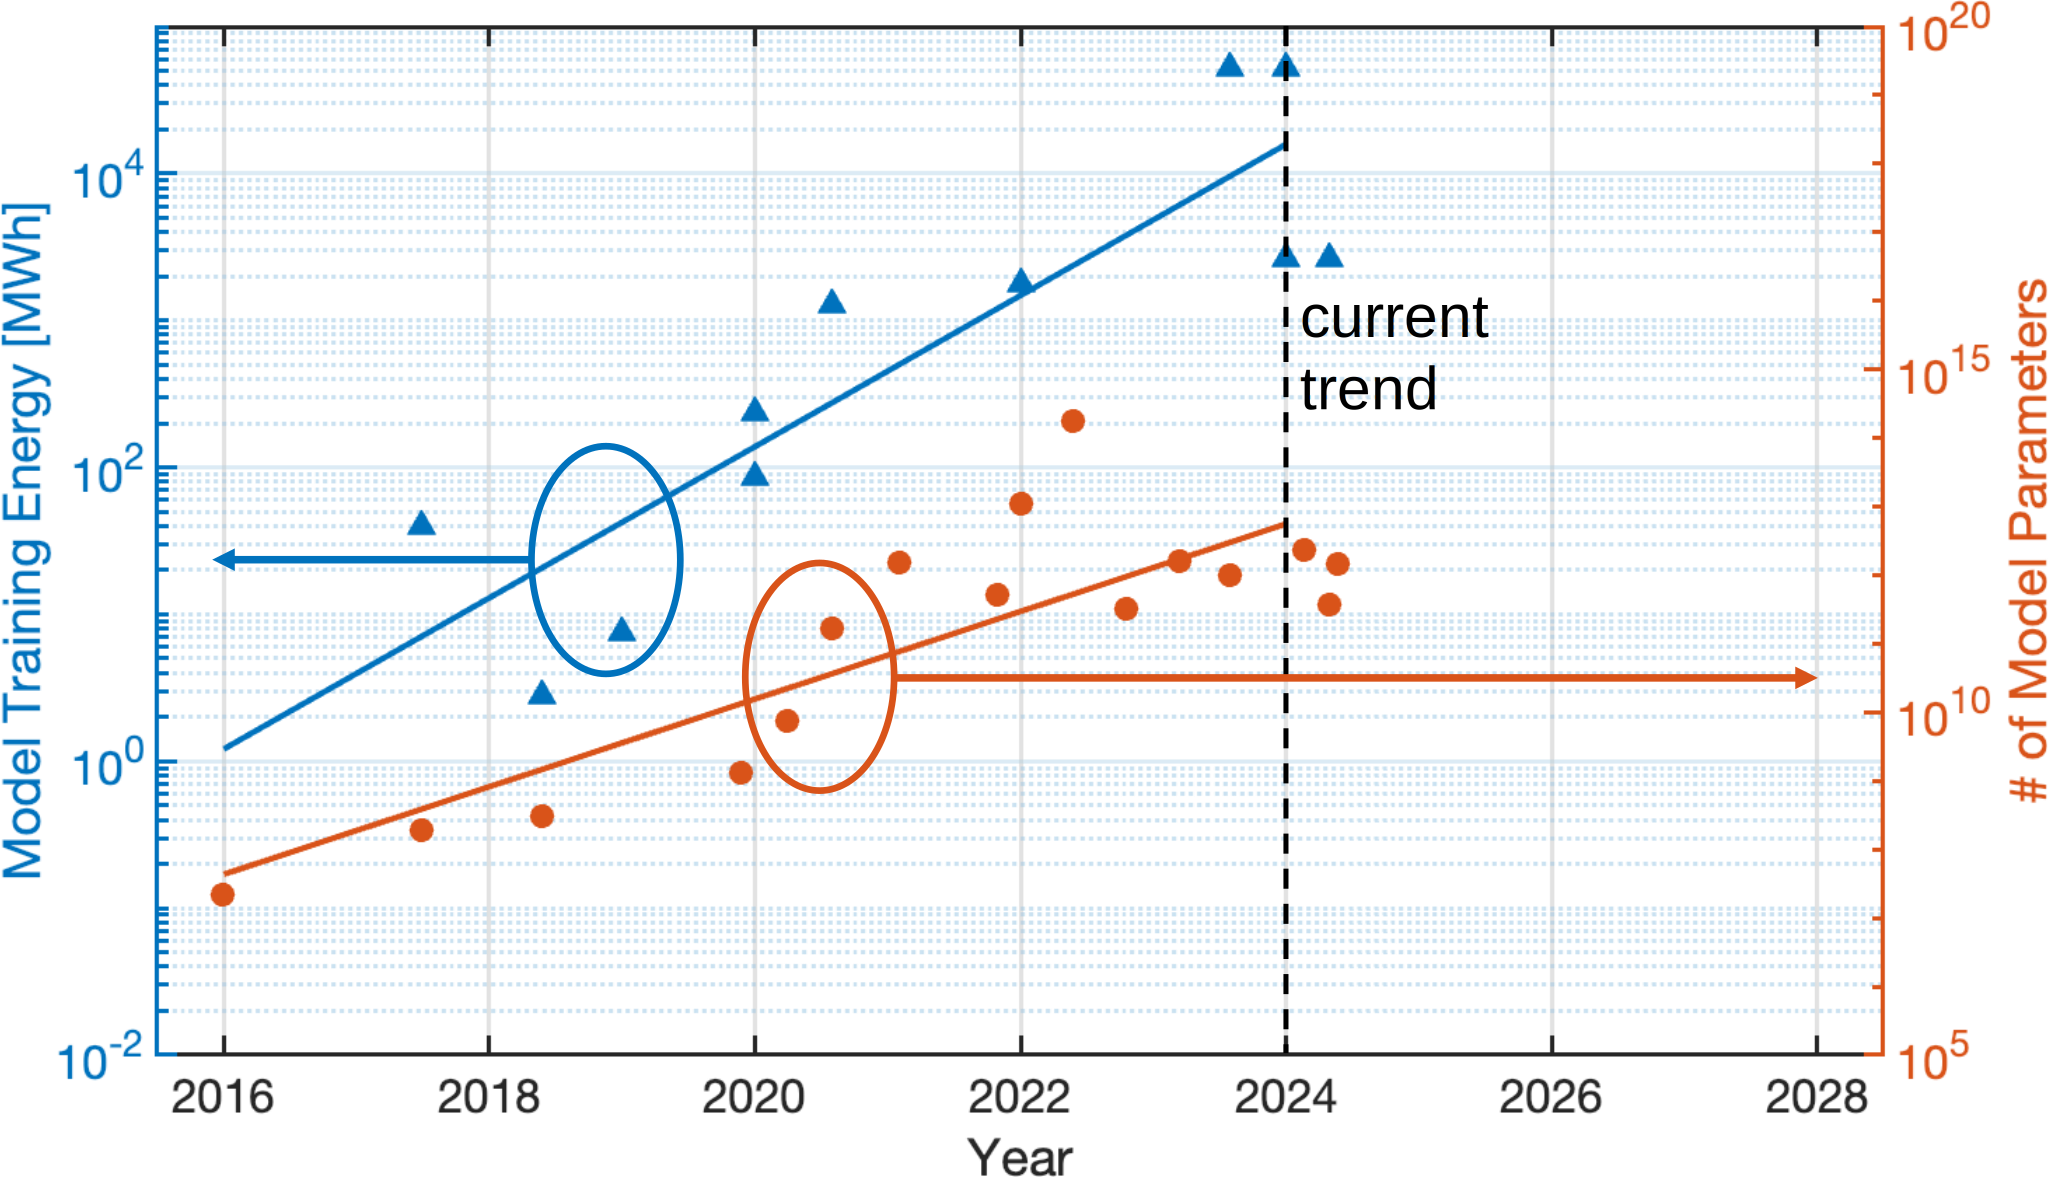
\includegraphics[width=0.75\textwidth]{fig/scaling-bend-1.pdf}}%
    \only<2-2>{\centering\includegraphics[width=0.75\textwidth]{fig/scaling-bend-2.pdf}}%
    \note<1-1>[item]{So, a quick summary, by empowering computing systems with both efficient data movement and data processing acceleration,}
    \note<2-2>[item]{my research aims to provide a mechanism to continue the scaling of AI computation, but at the same time, bending the energy curve, through the use of integrated photonics.}

\end{frame}
